% Provenance (never printed): old premiere S material on the structure of the
% Earth from seismology (P and S waves, travel times, the Moho, the shadow zone
% and the core, a reference model); see sources/book2/PROVENANCE.md. Profiles
% from figdata/grade-11/prem_profiles.py, rays and travel times from
% seismic_rays.py, the refraction lines and the problem's readings from
% moho_refraction.py. Lehmann's story and portrait are told in Book 1 (g6
% inside-the-earth): recalled here, not repeated.
\chapter{الموجات الزلزالية تكشف باطن الأرض}\label{ch:g11:seismic-structure}

في 8 أكتوبر 1909 هزّ زلزال وادي نهر كوبا، على بعد نحو
\qty{40}{km} جنوب شرق زغرب، في كرواتيا. وقبل ذلك ببضعة أشهر، كان أندريا
موهوروفيتشيتش قد ركّب مرسمة زلازل جديدة في مرصد زغرب
للأرصاد الجوية، فسجلت الحدث كله. ثم طلب من مراصد أخرى
سجلاتها فجمع سجلات 41 محطة. وعلى
سجلات المحطات الأبعد وجد شيئًا غير متوقع: موجتين P
منفصلتين، ضعيفة ثم أقوى منها، حيث كان ينبغي أن تكون
واحدة. ومن هذا الزوج من الموجات استنتج أن الصخر الذي تحت القشرة
مختلف، وقاس عمق الحد بينهما. يبيّن هذا الفصل
كيف تكشف الأزمنة التي تصل فيها موجات الزلازل طبقاتِ
الأرض: قاعدة القشرة، واللب وجزأه الخارجي السائل، والباطن
كله، عمقًا بعد عمق.
% ledger: herak:kupa-1909, srl:mohorovicic, geotech:moho-1909, kayal:pn-sn

\begin{recall}
يبدأ الزلزال عند نقطة داخل الأرض، هي البؤرة؛ والنقطة التي تعلوها مباشرة
على السطح هي المركز السطحي. ويسجل مقياس الزلازل اهتزاز
الأرض، ويقيس القدر حجم الزلزال (الكتاب 1،
الصف 7). وللأرض قشرة ووشاح ولب؛ وللب جزء خارجي
سائل وجزء داخلي صلب. وموجات الزلازل نوعان رئيسيان:
\omterm{def:g11:seismic-structure:body-waves}{الموجات P} الأسرع \omterm{def:g11:seismic-structure:body-waves}{والموجات S} الأبطأ، \omterm{def:g11:seismic-structure:body-waves}{والموجات S} لا تستطيع عبور سائل
(الكتاب 1، الصف 6). والموجة التي تعبر الحد بين مادتين
تنتقل فيهما بالسرعتين $v_1$ و$v_2$ تنكسر:
$\sin i_1/v_1 = \sin i_2/v_2$، حيث تقاس الزاويتان من
العمودي على الحد (قانون سنيل؛ كتب الفيزياء).
\end{recall}

\section{الموجات الزلزالية وأزمنة الانتقال}

\subsection{نوعان من الموجات الجسمية}

يرسل الزلزال موجات في كل الاتجاهات. بعضها ينتقل على امتداد السطح؛
وبعضها الآخر، أي الموجات الجسمية، ينتقل عبر باطن الأرض، وهي
التي تكشفه.

\begin{definition}[الموجة P؛ الموجة S]\label{def:g11:seismic-structure:body-waves}
\emph{الموجة P}\index{موجة P} موجة زلزالية تضغط الصخر وتمطه
على التناوب: فيتحرك الصخر ذهابًا وإيابًا على امتداد الاتجاه الذي
تنتقل فيه الموجة. وهي تعبر الأجسام الصلبة والسوائل والغازات، وهي
أسرع الموجات الزلزالية، فتصل أولًا. أما \emph{الموجة S}\index{موجة S}
فتقص الصخر: فيتحرك الصخر عموديًا على الاتجاه الذي تنتقل
فيه الموجة. ولا تعبر إلا الأجسام الصلبة، وتصل بعد الموجة P.
\end{definition}
% ledger: kayal:p-s

السائل ينساب ولا يقاوم تغيّر الشكل، فلا يستطيع
أن ينقل القص: ولهذا تتوقف \omterm{def:g11:seismic-structure:body-waves}{الموجات S} عند سطح السائل. وفي معظم
الصخور تنتقل \omterm{def:g11:seismic-structure:body-waves}{الموجة P} أسرع من \omterm{def:g11:seismic-structure:body-waves}{الموجة S} بنحو $\sqrt 3 \approx 1.7$ مرة.
ففي القشرة العليا تنتقل \omterm{def:g11:seismic-structure:body-waves}{الموجة P} بنحو \qty{5.8}{km/s} \omterm{def:g11:seismic-structure:body-waves}{والموجة S} بنحو
\qty{3.2}{km/s}؛ وتحت القشرة مباشرة تبلغان نحو
\qty{8.1}{km/s} و\qty{4.5}{km/s}.
% ledger: kayal:p-s, kayal:outer-core-liquid, data:prem (vp_surface 5.8, vs_surface 3.2,
% vp_upper_mantle 8.11, vs_upper_mantle 4.49 in figdata/grade-11/prem_profiles.py)

\begin{omfigure}

\includegraphics[width=0.5\linewidth]{images/book2/g11-usgs-seismometer.jpg}

{\small علماء زلازل من شبكة بورتوريكو الزلزالية ومن هيئة المسح الجيولوجي الأمريكية
يركّبون مقياس زلازل مؤقتًا في جنوب غرب بورتوريكو، في 10 يناير
2020. الصورة: توماس برات، هيئة المسح الجيولوجي الأمريكية (ملك عام).}
\end{omfigure}
% ledger: photo:g11-seismometer

\subsection{منحنيات زمن الانتقال}

تقاس المسافة من زلزال إلى محطة بعيدة على هيئة
زاوية: الزاوية $\Delta$ في مركز الأرض بين المركز السطحي
والمحطة، وهي \emph{المسافة المركزية}\index{مسافة مركزية}. والدرجة
الواحدة منها تساوي $\qty{111.2}{km}$ على امتداد السطح.
% ledger: earth:Rmean

\begin{definition}[زمن الانتقال؛ منحنى زمن الانتقال]\label{def:g11:seismic-structure:travel-time}
\emph{زمن الانتقال}\index{زمن الانتقال} لموجة زلزالية عند محطة هو
الزمن الذي تستغرقه للانتقال من البؤرة إلى المحطة. و\emph{منحنى زمن
الانتقال}\index{منحنى زمن الانتقال} لموجة هو التمثيل البياني
لزمن انتقالها بدلالة المسافة المركزية للمحطة.
\end{definition}

تسجل المحطة الزمن الذي تصل فيه كل موجة؛ وحين يكون زمن
الزلزال معروفًا، يكون الفرق هو \omterm{def:g11:seismic-structure:travel-time}{زمن الانتقال}. وقد أعطت آلاف
الزلازل التي سجلتها آلاف المحطات منحنيات \omterm{def:g11:seismic-structure:travel-time}{زمن الانتقال}
بدقة كبيرة. وفي الشكل حُسبت المنحنيات من
\omterm{def:g11:seismic-structure:reference-model}{النموذج المرجعي للأرض} في \cref{sec:g11:seismic-structure:model}، والنقاط
\omterm{def:g11:seismic-structure:travel-time}{أزمنة انتقال} رُصدت في زلازل حقيقية: ويتفق الاثنان في حدود
اثنين في المئة في كل مكان، وفي الغالب في حدود ثانية أو ثانيتين.

\begin{omfigure}
\begin{tikzpicture}
\begin{axis}[omrecord, width=0.84\linewidth, height=6.4cm, xmin=0, xmax=180, ymin=0, ymax=30,
  xtick={0,20,...,180}, ytick={0,5,...,30},
  xlabel={\foreignlanguage{arabic}{المسافة المركزية $\Delta$ بالدرجات}}, ylabel={\foreignlanguage{arabic}{زمن الانتقال بالدقائق}},
  tick label style={font=\small}, label style={font=\small}, clip=false]
% computed in figdata/grade-11/seismic_rays.py; ledger: data:prem, auspass:surftim
\addplot[omDef, line width=0.9pt] table[x=delta_deg, y=t_min] {figdata/out/grade-11-seismic_rays-ttp.dat};
\addplot[omProp, line width=0.9pt] table[x=delta_deg, y=t_min] {figdata/out/grade-11-seismic_rays-tts.dat};
\addplot[omDef, line width=0.9pt, densely dashed] table[x=delta_deg, y=t_min] {figdata/out/grade-11-seismic_rays-ttpkp.dat};
\addplot[omDef!55, line width=0.9pt, densely dotted] table[x=delta_deg, y=t_min] {figdata/out/grade-11-seismic_rays-ttpkikp.dat};
\addplot[only marks, mark=*, mark size=1.5pt, black] table[x=delta_deg, y=p_min] {figdata/out/grade-11-seismic_rays-observed.dat};
\addplot[only marks, mark=*, mark size=1.5pt, black, unbounded coords=discard] table[x=delta_deg, y=s_min] {figdata/out/grade-11-seismic_rays-observed.dat};
\node[font=\small, text=omProp, anchor=south east] at (axis cs:68,21.2) {S};
\node[font=\small, text=omDef, anchor=north west] at (axis cs:72,11.2) {P};
\node[font=\small, text=omDef, anchor=south, align=center] at (axis cs:158,23.2) {\foreignlanguage{arabic}{الموجة P}\\عبر اللب};
\fill[black!10] (axis cs:98.5,0) rectangle (axis cs:143.8,3.2);
\node[font=\scriptsize, align=center] at (axis cs:121.1,1.6) {\foreignlanguage{arabic}{لا موجة P مباشرة}};
\end{axis}
\end{tikzpicture}

{\small منحنيات \omterm{def:g11:seismic-structure:travel-time}{زمن الانتقال} \omterm{def:g11:seismic-structure:body-waves}{للموجات P} (بالأزرق) \omterm{def:g11:seismic-structure:body-waves}{والموجات S} (بالبرتقالي) من
زلزال عند السطح، محسوبة \omterm{def:g11:seismic-structure:reference-model}{بالنموذج المرجعي للأرض}؛ والمنحنيان المتقطع
والمنقّط موجتان P عبرتا اللب (المنقّط: اللب
الداخلي). النقاط السوداء: \omterm{def:g11:seismic-structure:travel-time}{أزمنة انتقال} مرصودة. وبين نحو \ang{99}
و\ang{144} لا تصل أي \omterm{def:g11:seismic-structure:body-waves}{موجة P} مباشرة (المنطقة المظللة).}
\end{omfigure}

يرتفع المنحنى S أشد انحدارًا من المنحنى P، فيزداد التأخر بين
الوصولين مع المسافة. وهذا يعطي بعد الزلزال انطلاقًا من
سجل واحد.

\begin{method}[بعد الزلزال من التأخر S--P]\label{met:g11:seismic-structure:distance}
\begin{enumerate}
  \item على السجل، اقرأ زمن وصول أول \omterm{def:g11:seismic-structure:body-waves}{موجة P} وأول \omterm{def:g11:seismic-structure:body-waves}{موجة
        S}؛ والفرق بينهما هو التأخر S--P.
  \item على منحنيات \omterm{def:g11:seismic-structure:travel-time}{زمن الانتقال} (أو في جدول لها)، جد
        المسافة المركزية التي يقع عندها المنحنى S فوق المنحنى P
        بذلك التأخر.
  \item حوّل إلى الكيلومترات، عند الحاجة، بمعدل $\qty{111.2}{km}$ لكل درجة.
\end{enumerate}
وبثلاث محطات، يكون المركز السطحي هو النقطة التي تقع على البعد الصحيح من
الثلاث كلها.
\end{method}

\begin{example}[زلزال على بعد \ang{60}]\label{ex:g11:seismic-structure:sp}
\omterm{def:g11:seismic-structure:travel-time}{أزمنة الانتقال} المرصودة \qty{608}{s} \omterm{def:g11:seismic-structure:body-waves}{للموجة P} و\qty{1101}{s} \omterm{def:g11:seismic-structure:body-waves}{للموجة S} عند
\ang{60}، و\qty{536}{s} و\qty{967}{s} عند \ang{50}. فالمحطة التي تسجل
\omterm{def:g11:seismic-structure:body-waves}{موجة S} بعد \omterm{def:g11:seismic-structure:body-waves}{الموجة P} بمقدار \qty{493}{s} (8~دقائق و13~ثانية)
تقع إذن على بعد \ang{60} من المركز السطحي: أي نحو $60 \times 111.2 \approx
\qty{6670}{km}$. وعند \ang{50} لن يتجاوز التأخر \qty{431}{s}.
\end{example}
% ledger: auspass:surftim

\begin{omfigure}
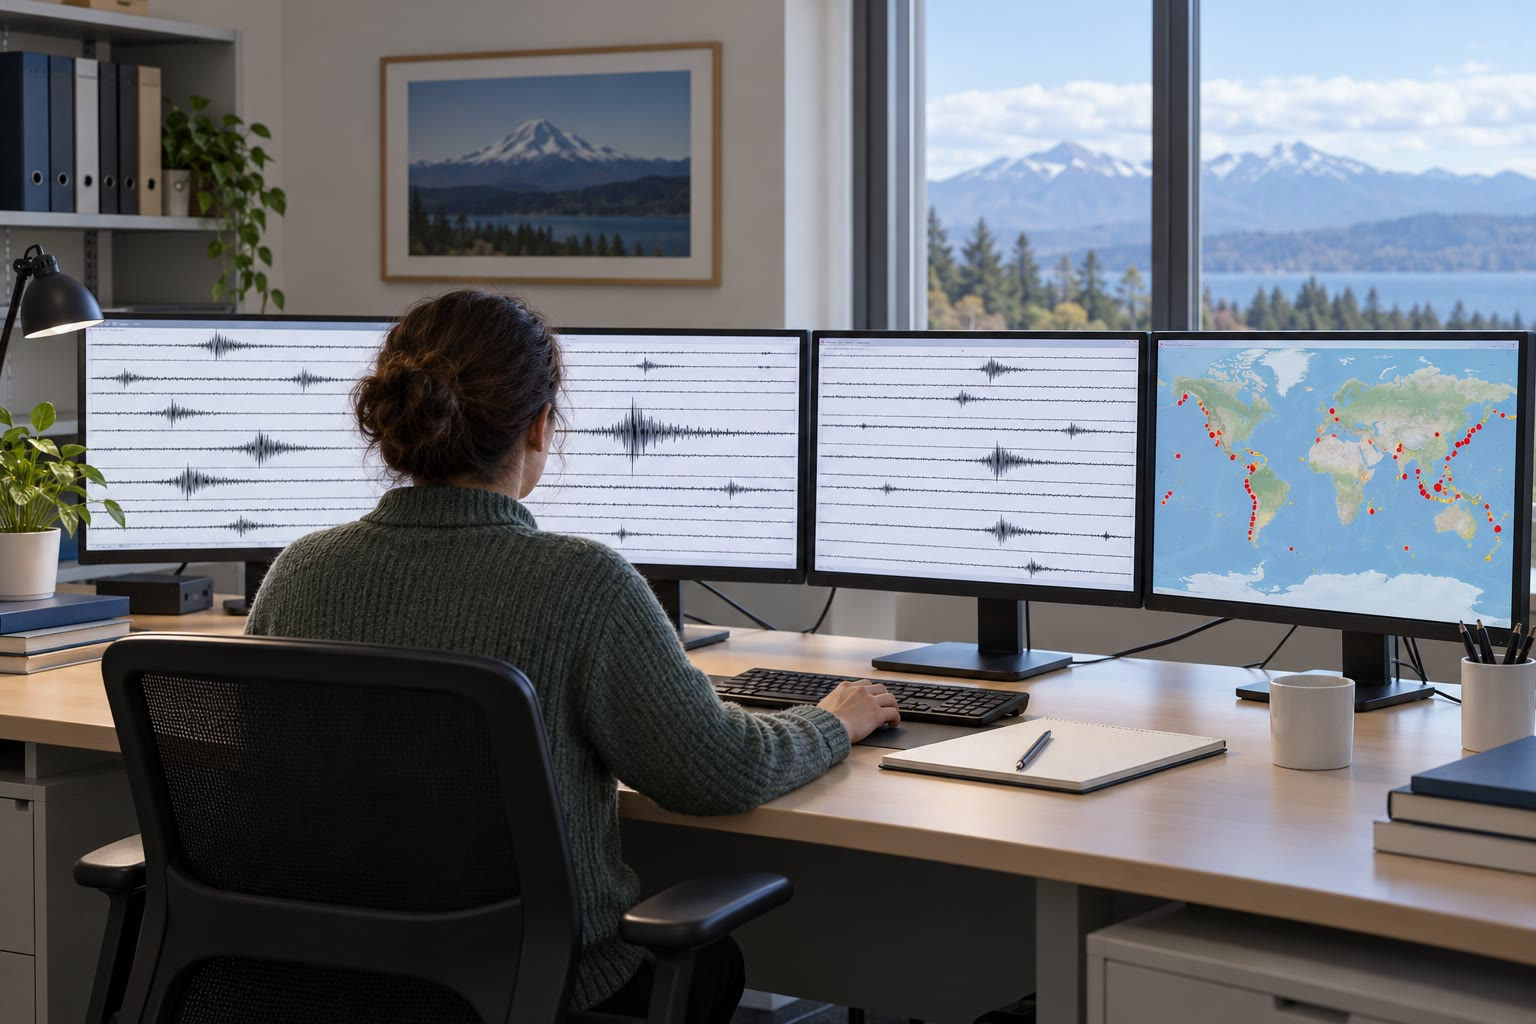
\includegraphics[width=0.66\linewidth]{images/book2/ai/g11-seismology-observatory.jpg}

{\small في مرصد لعلم الزلازل، تُعرض سجلات محطات كثيرة
جنبًا إلى جنب، وتُرسم الزلازل التي تحدد مواقعها على خريطة للعالم
(صورة مولدة بالذكاء الاصطناعي).}
\end{omfigure}

\section{الانكسار والموهو}\label{sec:g11:seismic-structure:moho}

\subsection{الموجة التي تجري على امتداد حد}

تتغير سرعة الموجات الزلزالية داخل الأرض مع العمق، تدريجيًا في
الغالب، لكنها تتغير في بعض المواضع دفعة واحدة.

\begin{definition}[الانقطاع الزلزالي]\label{def:g11:seismic-structure:discontinuity}
\emph{الانقطاع الزلزالي}\index{انقطاع زلزالي} سطح
داخل الأرض تتغير عبره سرعة الموجات الزلزالية
فجأة --- على سمك أصغر بكثير من طول الموجات.
\end{definition}

عند الانقطاع ينعكس جزء من الموجة وينكسر جزء آخر. لنأخذ
طبقة سمكها $h$ تنتقل فيها \omterm{def:g11:seismic-structure:body-waves}{الموجات P} بالسرعة $v_1$، فوق طبقة
تكون فيها أسرع، $v_2 > v_1$. فالشعاع الهابط بالزاوية $i$ عن
الرأسي ينكسر بالزاوية $r$ المعطاة بالعلاقة $\sin r = (v_2/v_1)\sin
i$: أي إنه ينحرف مبتعدًا عن الرأسي. وحين تبلغ $\sin i$ القيمة $v_1/v_2$، يجري
الشعاع المنكسر على امتداد الحد تمامًا. والزاوية
\[
  i_c, \qquad \sin i_c = \frac{v_1}{v_2},
\]
هي \emph{الزاوية الحدية}\index{زاوية حدية}. والموجة المنكسرة \omterm{ex:g11:seismic-structure:sp}{بالزاوية
الحدية} تنتقل على امتداد أعلى الطبقة الأسرع بالسرعة $v_2$،
وهي في أثناء ذلك ترسل موجات صاعدة إلى الطبقة العليا، كلها بالزاوية
$i_c$: فتصل إلى السطح على هيئة \emph{الموجة المنكسرة الحرجة}\index{موجة منكسرة حرجة}.

\begin{omfigure}
\begin{tikzpicture}[x=0.05cm, y=0.05cm, font=\footnotesize, >={Stealth[length=4pt]}]
% geometry from figdata/grade-11/moho_refraction.py: v1 6.2, v2 8.1, h 30 km, ic 49.9 deg
  \fill[omLithGranite!45] (-10,0) rectangle (215,-30);
  \fill[omLithPeridotite!45] (-10,-30) rectangle (215,-48);
  \draw[line width=0.6pt] (-10,0) -- (215,0);
  \draw[line width=0.9pt] (-10,-30) -- (215,-30);
  \node[anchor=west, align=left] at (218,-15) {القشرة\\$v_1 = \qty{6.2}{km/s}$};
  \node[anchor=west, align=left] at (218,-39) {الوشاح\\$v_2 = \qty{8.1}{km/s}$};
  \node[anchor=east] at (215,-26) {الموهو};
  % source and station
  \fill[omDef] (0,0) circle (1.6);
  \node[anchor=south] at (0,1.5) {الزلزال};
  \draw[fill=white] (197,0) -- (203,0) -- (200,5) -- cycle;
  \node[anchor=south] at (200,5) {المحطة};
  % direct wave
  \draw[->, omProp, line width=0.8pt] (2,-2) -- (196,-2);
  \node[anchor=south, text=omProp] at (100,0.3) {\foreignlanguage{arabic}{الموجة المباشرة، بالسرعة $v_1$}};
  % head wave
  \draw[omDef, line width=0.9pt] (0,0) -- (35.7,-30);
  \draw[->, omDef, line width=0.9pt] (35.7,-30) -- (100,-30);
  \draw[omDef, line width=0.9pt] (100,-30) -- (164.3,-30) -- (200,0);
  \node[anchor=north, text=omDef] at (100,-31) {\foreignlanguage{arabic}{على امتداد الموهو بالسرعة $v_2$}};
  \foreach \x in {50,70,90,110,130,150} {
    \draw[->, omDef!60, densely dashed] (\x,-30) -- ++(25.5,21.5);
  }
  % critical angle
  \draw[black!60, densely dotted] (35.7,-30) -- (35.7,-8);
  \draw[black!70] (35.7,-18) arc[start angle=90, end angle=130.05, radius=12];
  \node[anchor=south east] at (33,-16) {$i_c$};
  % thickness and critical distance
  \draw[<->] (-6,0) -- (-6,-30);
  \node[anchor=east] at (-7,-15) {$h$};
\end{tikzpicture}

{\small الموجة المباشرة \omterm{ex:g11:seismic-structure:sp}{والموجة المنكسرة الحرجة} (بمقياس رسم حقيقي: قشرة سمكها \qty{30}{km}).
تهبط \omterm{ex:g11:seismic-structure:sp}{الموجة المنكسرة الحرجة} \omterm{ex:g11:seismic-structure:sp}{بالزاوية الحدية} $i_c$، وتجري على امتداد
أعلى الوشاح ثم تصعد بالزاوية $i_c$؛ وعلى طول مسارها كله على
\omterm{def:g11:seismic-structure:moho}{الموهو} ترسل موجات صاعدة إلى السطح (الخطوط المتقطعة). ولا تصل إلى أي محطة أقرب
من $2h\tan i_c$، أي نحو \qty{71}{km} هنا.}
\end{omfigure}

\begin{proposition}[زمن انتقال الموجة المنكسرة الحرجة]\label{prop:g11:seismic-structure:head-wave}
لمصدر عند السطح، تتلقى المحطة الواقعة على المسافة $x \ge 2h\tan i_c$
\omterm{ex:g11:seismic-structure:sp}{الموجة المنكسرة الحرجة} بعد
\[
  t(x) = \frac{x}{v_2} + \frac{2h\cos i_c}{v_1}.
\]
ومنحنى زمن انتقالها مستقيم ميله $1/v_2$، إذا مُدّ
إلى الوراء قطع محور الزمن عند \emph{زمن التقاطع}\index{زمن التقاطع}
$t_i = 2h\cos i_c/v_1$.
\end{proposition}

\begin{proof}
يهبط الشعاع على ضلع مائل طوله $h/\cos i_c$، يتقدم به
أفقيًا بمقدار $h\tan i_c$؛ ويفعل الشيء نفسه في الصعود. وبينهما
يجري على امتداد الحد مسافة $x - 2h\tan i_c$. فالزمن هو
\[
  t = \frac{2h}{v_1\cos i_c} + \frac{x - 2h\tan i_c}{v_2}
    = \frac{x}{v_2} + \frac{2h}{v_1\cos i_c} - \frac{2h\sin i_c}{v_2\cos i_c}.
\]
وبما أن $1/v_2 = \sin i_c/v_1$، فإن الحدين الأخيرين يعطيان
$\frac{2h}{v_1\cos i_c}\,(1 - \sin^2 i_c) = \frac{2h\cos i_c}{v_1}$.
\end{proof}

تصل الموجة المباشرة بعد $x/v_1$: فمنحناها مستقيم يمر
بالأصل، أشد انحدارًا من مستقيم \omterm{ex:g11:seismic-structure:sp}{الموجة المنكسرة الحرجة}. فقرب المصدر تصل الموجة المباشرة
أولًا؛ وبعيدًا عنه تسبقها \omterm{ex:g11:seismic-structure:sp}{الموجة المنكسرة الحرجة}، التي قطعت معظم الطريق بالسرعة
الأعلى.

\begin{proposition}[مسافة العبور]\label{prop:g11:seismic-structure:crossover}
تصل \omterm{ex:g11:seismic-structure:sp}{الموجة المنكسرة الحرجة} قبل الموجة المباشرة فيما وراء \emph{مسافة
العبور}\index{مسافة العبور}
\[
  x_c = 2h\sqrt{\frac{v_2 + v_1}{v_2 - v_1}}.
\]
\end{proposition}

\begin{proof}
تصل الموجتان معًا حين يكون $x/v_1 = x/v_2 + 2h\cos i_c/v_1$، أي
$x\,(v_2 - v_1)/(v_1 v_2) = 2h\cos i_c/v_1$، ومنه $x = 2h\cos i_c\,v_2/(v_2 -
v_1)$. والآن $\cos i_c = \sqrt{1 - v_1^2/v_2^2} = \sqrt{(v_2 - v_1)(v_2 +
v_1)}/v_2$، ومن ثم $x = 2h\sqrt{(v_2 + v_1)(v_2 - v_1)}/(v_2 - v_1) =
2h\sqrt{(v_2 + v_1)/(v_2 - v_1)}$. وفيما وراءها تصل أولًا \omterm{ex:g11:seismic-structure:sp}{الموجة المنكسرة الحرجة}، التي
مستقيمها أقل انحدارًا.
\end{proof}

\begin{omfigure}
\begin{tikzpicture}
\begin{axis}[omrecord, width=0.78\linewidth, height=5.6cm, xmin=0, xmax=300, ymin=0, ymax=50,
  xtick={0,50,...,300}, xlabel={\foreignlanguage{arabic}{البعد عن المركز السطحي \babelsublr{(\unit{km})}}}, ylabel={\foreignlanguage{arabic}{زمن الانتقال \babelsublr{(\unit{s})}}},
  tick label style={font=\small}, label style={font=\small}, clip=false]
% computed in figdata/grade-11/moho_refraction.py (critical_km 71.4, crossover_km 164.6, intercept_s 6.23)
\addplot[omProp, line width=0.9pt] table[x=x, y=tdirect] {figdata/out/grade-11-moho_refraction-model.dat};
\addplot[omDef, line width=0.9pt, restrict x to domain=71:300] table[x=x, y=thead] {figdata/out/grade-11-moho_refraction-model.dat};
\addplot[omDef, densely dashed, restrict x to domain=0:72] table[x=x, y=thead] {figdata/out/grade-11-moho_refraction-model.dat};
\draw[black!50, densely dotted] (axis cs:164.6,0) -- (axis cs:164.6,26.5);
\node[font=\scriptsize, anchor=north] at (axis cs:164.6,0) {$x_c$};
\fill (axis cs:0,6.23) circle (1.5pt);
\draw[black!60] (axis cs:0.8,6.6) -- (axis cs:6,12);
\node[font=\scriptsize, anchor=south west, inner sep=1pt] at (axis cs:5,12) {$t_i = \qty{6.2}{s}$};
\node[font=\small, text=omProp, anchor=south east] at (axis cs:250,41) {الموجة المباشرة};
\node[font=\small, text=omDef, anchor=north west] at (axis cs:235,33) {الموجة المنكسرة الحرجة};
\end{axis}
\end{tikzpicture}

{\small \omterm{def:g11:seismic-structure:travel-time}{أزمنة انتقال} الموجة المباشرة \omterm{ex:g11:seismic-structure:sp}{والموجة المنكسرة الحرجة} للقشرة
في الشكل السابق. ومستقيم \omterm{ex:g11:seismic-structure:sp}{الموجة المنكسرة الحرجة}، إذا مُدّ إلى الوراء (المتقطع)، يقطع
محور الزمن عند \omterm{prop:g11:seismic-structure:head-wave}{زمن التقاطع}؛ وفيما وراء \omterm{prop:g11:seismic-structure:crossover}{مسافة العبور} $x_c \approx
\qty{165}{km}$ تصل \omterm{ex:g11:seismic-structure:sp}{الموجة المنكسرة الحرجة} أولًا.}
\end{omfigure}

\subsection{قاعدة القشرة}

\begin{definition}[الموهو]\label{def:g11:seismic-structure:moho}
\emph{انقطاع موهوروفيتشيتش}\index{انقطاع موهوروفيتشيتش}، أو
\emph{الموهو}\index{موهو}، هو \omterm{def:g11:seismic-structure:discontinuity}{الانقطاع الزلزالي} عند قاعدة
القشرة، حيث تقفز سرعة \omterm{def:g11:seismic-structure:body-waves}{الموجات P} من نحو \qty{7}{km/s} على الأكثر
إلى نحو \qty{8}{km/s}، وهي السرعة في أعلى الوشاح.
\end{definition}
% ledger: kayal:pn-sn, data:prem (6.8 -> 8.11 at 24.4 km)

\begin{history}[موهوروفيتشيتش والموجتان P، 1909]
وجد أندريا موهوروفيتشيتش (1857--1936)، في سجلات زلزال
عام 1909، أنه فيما وراء مسافة معينة --- بين 100 و\qty{150}{km}
عمومًا --- كانت \omterm{def:g11:seismic-structure:body-waves}{موجة P} ضعيفة وأسرع تصل قبل \omterm{def:g11:seismic-structure:body-waves}{الموجة P} القوية.
وفسّرها بأنها موجة انتقلت عبر صخر أسرع تحت
القشرة. وسمّى الموجتين Pg (الموجة المباشرة في القشرة) وPn (\omterm{ex:g11:seismic-structure:sp}{الموجة
المنكسرة الحرجة} على امتداد أعلى الوشاح)، وفعل الشيء نفسه مع \omterm{def:g11:seismic-structure:body-waves}{الموجات S}،
واستنتج سرعتي الطبقتين وعمق الحد بينهما.
وتنتقل الموجة Pn بنحو \qty{8.0}{km/s}، وهي سرعة أعلى
الوشاح. وقد أثبتت أبحاثه المنشورة عام 1910 أن القشرة والوشاح
مختلفان؛ ويحمل الحد بينهما اسمه.
\end{history}
% ledger: kayal:pn-sn, srl:mohorovicic

\begin{method}[عمق الموهو من مخطط أزمنة الانتقال]\label{met:g11:seismic-structure:moho}
\begin{enumerate}
  \item ارسم أزمنة الوصول الأولى بدلالة البعد عن
        المركز السطحي.
  \item ارسم مستقيم الموجة المباشرة (المار بالأصل) ومستقيم
        \omterm{ex:g11:seismic-structure:sp}{الموجة المنكسرة الحرجة}؛ ميلاهما $1/v_1$ و$1/v_2$.
  \item مدّ مستقيم \omterm{ex:g11:seismic-structure:sp}{الموجة المنكسرة الحرجة} إلى الوراء حتى محور الزمن: فيقطعه عند
        \omterm{prop:g11:seismic-structure:head-wave}{زمن التقاطع} $t_i$.
  \item بما أن $\sin i_c = v_1/v_2$، فسمك القشرة هو
        $h = \dfrac{v_1\,t_i}{2\cos i_c}$.
\end{enumerate}
\end{method}

\begin{example}[قشرة سمكها \qty{30}{km}]\label{ex:g11:seismic-structure:moho}
مع $v_1 = \qty{6.2}{km/s}$ و$v_2 = \qty{8.1}{km/s}$، يكون $\sin i_c = 0.765$،
و$i_c \approx \ang{49.9}$ و$\cos i_c \approx 0.644$. وزمن تقاطع قدره
\qty{6.23}{s} يعطي $h = 6.2 \times 6.23/(2 \times 0.644) \approx
\qty{30}{km}$. وتصل \omterm{ex:g11:seismic-structure:sp}{الموجة المنكسرة الحرجة} إلى السطح أول مرة عند
$2h\tan i_c \approx \qty{71}{km}$ وتسبق الموجة المباشرة فيما وراء
$x_c = 60\sqrt{14.3/1.9} \approx \qty{165}{km}$.
\end{example}
% values computed in figdata/grade-11/moho_refraction.py (ic_deg 49.9, critical_km 71.4, crossover_km 164.6)

إذا قيس \omterm{def:g11:seismic-structure:moho}{الموهو} بهذه الطريقة في أنحاء العالم كله، وُجد أنه لا يقع إلا على عمق نحو
\qty{5}{km} تحت قاع المحيطات. أما تحت القارات فيقع على عمق نحو
\qty{41}{km} في المتوسط: نحو \qty{30}{km} حيث
مُطّت القشرة، وأكثر من \qty{45}{km} تحت الأحزمة الجبلية، وحتى نحو
\qty{100}{km} تحت أعلى السلاسل. فالقشرة جلد رقيق: حتى
\qty{41}{km} أقل من واحد في المئة من نصف قطر الأرض.
% ledger: usgs:crust-thickness, cm95:crust, kayal:discontinuities

\section{اللب}

\subsection{أشعة تنحني}

تزداد سرعة الموجات الزلزالية في الوشاح مع العمق. فالشعاع
الهابط يعبر صخرًا أسرع فأسرع، فينحرف، بحسب قانون سنيل،
مبتعدًا قليلًا عن الرأسي عند كل خطوة: فينحني مساره ويرتد
صاعدًا نحو السطح. وكلما كان ارتداد الشعاع أعمق، عاد إلى السطح أبعد عن
الزلزال. ويبيّن الشكل أشعة كهذه، محسوبة بسرعات
\omterm{def:g11:seismic-structure:reference-model}{النموذج المرجعي للأرض}.

\begin{omfigure}
\begin{tikzpicture}
\begin{axis}[width=0.66\linewidth, height=0.66\linewidth, axis equal image, hide axis,
  xmin=-1.18, xmax=1.18, ymin=-1.18, ymax=1.2, clip=false]
% computed in figdata/grade-11/seismic_rays.py; ledger: data:prem
\fill[omLithPeridotite!25] (axis cs:0,0) circle [radius=1];
\fill[omSea!45] (axis cs:0,0) circle [radius=0.5462];
\fill[omSea!80] (axis cs:0,0) circle [radius=0.1917];
\addplot[black, line width=0.6pt, domain=0:360, samples=181] ({cos(x)}, {sin(x)});
\addplot[black!60, line width=0.4pt, domain=0:360, samples=181] ({0.5462*cos(x)}, {0.5462*sin(x)});
\addplot[black!60, line width=0.4pt, domain=0:360, samples=91] ({0.1917*cos(x)}, {0.1917*sin(x)});
\addplot[omDef, line width=0.6pt] table {figdata/out/grade-11-seismic_rays-praysmantle.dat};
\addplot[omDef!70!black, line width=0.6pt] table {figdata/out/grade-11-seismic_rays-prayscore.dat};
\addplot[omProp, line width=0.6pt] table {figdata/out/grade-11-seismic_rays-srays.dat};
% P shadow zone: 98.5 to 143.8 degrees from the source (right); S beyond 102.7 (left)
\addplot[black!80, line width=3pt, domain=-53.8:-8.5, samples=40] ({1.04*cos(x)}, {1.04*sin(x)});
\addplot[omProp!60, line width=3pt, domain=192.7:270, samples=40] ({1.04*cos(x)}, {1.04*sin(x)});
\fill[omDef] (axis cs:0,1) circle (2pt);
\node[font=\footnotesize, anchor=south] at (axis cs:0,1.04) {الزلزال};
\node[font=\footnotesize, anchor=west, align=left] at (axis cs:1.07,-0.42) {\foreignlanguage{arabic}{لا موجة P مباشرة}\\(\ang{99}--\ang{144})};
\node[font=\footnotesize, anchor=east, align=right] at (axis cs:-1.07,-0.62) {\foreignlanguage{arabic}{لا موجة S مباشرة}\\\foreignlanguage{arabic}{بعد \babelsublr{\ang{103}}}};
\node[font=\footnotesize, text=omDef, anchor=south west] at (axis cs:0.55,0.8) {P};
\node[font=\footnotesize, text=omProp, anchor=south east] at (axis cs:-0.55,0.8) {S};
\node[font=\scriptsize] at (axis cs:-0.5,-0.62) {الوشاح};
\node[font=\scriptsize] at (axis cs:-0.3,0.2) {اللب الخارجي};
\draw[black!70] (axis cs:-0.1,-0.06) -- (axis cs:-0.26,-0.22);
\node[font=\scriptsize, anchor=north east, inner sep=1pt] at (axis cs:-0.24,-0.22) {اللب الداخلي};
\end{axis}
\end{tikzpicture}

{\small أشعة من زلزال في أعلى الأرض، محسوبة
بسرعات النموذج المرجعي. في اليمين: أشعة P ترتد في الوشاح، حتى
نحو \ang{99}، وأشعة P تعبر اللب وتخرج فيما وراء نحو
\ang{144}؛ وبينهما لا يصل أي شعاع P مباشرة. في اليسار: أشعة S، التي ترتد في
الوشاح؛ ولا يعبر أي منها اللب الخارجي السائل، ولا تصل أي \omterm{def:g11:seismic-structure:body-waves}{موجة S} مباشرة إلى
ما وراء نحو \ang{103}.}
\end{omfigure}

\subsection{منطقة الظل واللب الخارجي السائل}

في عام 1906 لاحظ عالم الزلازل أولدهام أن \omterm{def:g11:seismic-structure:body-waves}{الموجات P} المسجلة على الجانب البعيد
من الأرض عن الزلزال تصل متأخرة عن الأزمنة
المتوقعة، فاقترح لبًّا مركزيًا تنتقل فيه أبطأ. وفي
عام 1912 بيّن غوتنبرغ أن \omterm{def:g11:seismic-structure:body-waves}{الموجات P} لا تصل إلى نطاق كامل من المسافات،
بين نحو \ang{105} و\ang{143}، مع وصول قوي فيما وراء
\ang{143} مباشرة؛ وفي عام 1914 حدّد أعلى اللب على عمق \qty{2900}{km}.
% ledger: kayal:discontinuities, kayal:shadow

\begin{definition}[منطقة الظل]\label{def:g11:seismic-structure:shadow-zone}
\emph{منطقة الظل}\index{منطقة الظل} لموجة زلزالية هي مدى
المسافات المركزية الذي لا تستطيع الموجة بلوغه مباشرة من
الزلزال، لأن اللب يحرفها عنه أو يوقفها.
\end{definition}

تفسرها الأشعة. فأشعة P التي ترتد فوق اللب مباشرة تعود صاعدة
على بعد نحو \ang{100} من الزلزال. والشعاع الذي يهبط أشد انحدارًا قليلًا
يدخل اللب، حيث تهبط سرعة \omterm{def:g11:seismic-structure:body-waves}{الموجة P} فجأة من \qty{13.7}{km/s} إلى
نحو \qty{8.1}{km/s}: فينحرف، بحسب قانون سنيل، \emph{نحو} الرأسي،
ويعبر اللب ويخرج أبعد بكثير، فيما وراء نحو \ang{144}. ولا يحط بينهما أي
شعاع P يرتد في الوشاح ولا أي شعاع P يعبر اللب.
وفي النموذج المرجعي تمتد منطقة ظل \omterm{def:g11:seismic-structure:body-waves}{الموجات P} من \ang{98.5} إلى
\ang{143.8}، قريبًا من قيمتي غوتنبرغ \ang{105}--\ang{143}.
% ledger: kayal:shadow, data:prem (vp_above_cmb 13.72, vp_below_cmb 8.06); computed in
% figdata/grade-11/seismic_rays.py (shadow_start_deg 98.5, shadow_end_pkp_deg 143.8)

وتخبرنا \omterm{def:g11:seismic-structure:body-waves}{الموجات S} بأكثر من ذلك. فلا تعبر أي \omterm{def:g11:seismic-structure:body-waves}{موجة S} اللب الخارجي: إن اللب الخارجي لا
ينقل موجات القص، فهو إذن سائل. ونتيجة لذلك لا تصل أي \omterm{def:g11:seismic-structure:body-waves}{موجة S} مباشرة
فيما وراء نحو \ang{103} في النموذج المرجعي --- أي على الجانب البعيد كله من
الأرض.
% ledger: kayal:outer-core-liquid; computed in figdata/grade-11/seismic_rays.py (s_direct_max_deg 102.7)

\begin{definition}[الحد بين اللب والوشاح؛ حد اللب الداخلي]\label{def:g11:seismic-structure:core}
\emph{الحد بين اللب والوشاح}\index{حد بين اللب والوشاح} هو \omterm{def:g11:seismic-structure:discontinuity}{الانقطاع
الزلزالي} بين الوشاح الصلب واللب الخارجي السائل، على عمق
\qty{2891}{km}؛ وعنده تهبط سرعة \omterm{def:g11:seismic-structure:body-waves}{الموجة P} من نحو \qty{13.7}{km/s} إلى
نحو \qty{8.1}{km/s}، وتتوقف \omterm{def:g11:seismic-structure:body-waves}{الموجات S}. أما \emph{حد اللب
الداخلي}\index{حد اللب الداخلي}، على عمق \qty{5150}{km}، فيفصل
اللب الخارجي السائل عن اللب الداخلي الصلب؛ وعنده تقفز سرعة \omterm{def:g11:seismic-structure:body-waves}{الموجة P} من
نحو \qty{10.4}{km/s} إلى نحو \qty{11.0}{km/s}.
\end{definition}
% ledger: data:prem, prem:cmb, prem:icb (Book 3 rows); values in figdata/grade-11/prem_profiles.py

ليست \omterm{def:g11:seismic-structure:shadow-zone}{منطقة الظل} صامتة تمامًا: \omterm{def:g11:seismic-structure:body-waves}{فموجات P} ضعيفة تصل إليها. وقد فسّرتها إنغه
ليمان عام 1936 بلب داخلي صلب تنتقل فيه \omterm{def:g11:seismic-structure:body-waves}{الموجات P}
أسرع (الكتاب 1، الصف 6). وتبيّن الأشعة كيف. فشعاع P الذي يبلغ
اللب الداخلي ينحرف مبتعدًا عن الرأسي حيث تقفز السرعة صعودًا، كما عند
\omterm{def:g11:seismic-structure:moho}{الموهو}، فيخرج من اللب أبكر: ففي النموذج المرجعي تبلغ الأشعة
العابرة للب الداخلي السطح ابتداءً من نحو \ang{121}، داخل
\omterm{def:g11:seismic-structure:shadow-zone}{منطقة الظل} (المنحنى المنقّط في شكل \omterm{def:g11:seismic-structure:travel-time}{أزمنة الانتقال}).
% ledger: nbi:lehmann-1936 (Book 1 row), kayal:lehmann; computed in
% figdata/grade-11/seismic_rays.py (pkikp_min_deg 121.4)

\section{نموذج مرجعي للأرض}\label{sec:g11:seismic-structure:model}

إذا جُمعت ملايين \omterm{def:g11:seismic-structure:travel-time}{أزمنة الانتقال} أعطت سرعة \omterm{def:g11:seismic-structure:body-waves}{الموجات P} وS عند
كل عمق. وسرعاتها تتوقف على الصخر وعلى كثافته، والكتلة
الكلية للأرض تحدد متوسط كثافتها؛ فيعطيان معًا
الكثافة عند كل عمق أيضًا.
% ledger: data:prem, prem:constraints (Book 3 row)

\begin{definition}[النموذج المرجعي للأرض]\label{def:g11:seismic-structure:reference-model}
\emph{النموذج المرجعي للأرض}\index{نموذج مرجعي للأرض} جدول
لسرعة \omterm{def:g11:seismic-structure:body-waves}{الموجات P} وسرعة \omterm{def:g11:seismic-structure:body-waves}{الموجات S} والكثافة بدلالة العمق، متماثل
في كل الاتجاهات، يُختار ليتفق مع \omterm{def:g11:seismic-structure:travel-time}{أزمنة الانتقال} المرصودة
للموجات الزلزالية ومع كتلة الأرض.
\end{definition}

وأكثرها استعمالًا النموذج المرجعي الأولي للأرض (PREM)، الذي نشره
أ.~م.~جيفونسكي ود.~ل.~أندرسون عام 1981. وقد حُسبت به أشعة هذا
الفصل وأزمنة انتقاله: \omterm{def:g11:seismic-structure:travel-time}{فزمن انتقال} \omterm{def:g11:seismic-structure:body-waves}{الموجة P} عند \ang{60}، مثلًا،
يخرج \qty{607}{s}، مقابل \qty{608}{s} مرصودة.
% ledger: data:prem, auspass:surftim; computed in figdata/grade-11/seismic_rays.py (p_60_s 607.2)

\begin{omfigure}
\begin{tikzpicture}
\begin{axis}[omrecord, width=0.86\linewidth, height=6.2cm, xmin=0, xmax=6371, ymin=0, ymax=14.5,
  xtick={0,1000,...,6000}, ytick={0,2,...,14}, scaled x ticks=false,
  xticklabel style={/pgf/number format/1000 sep={\,}},
  xlabel={\foreignlanguage{arabic}{العمق \babelsublr{(\unit{km})}}}, ylabel={\foreignlanguage{arabic}{السرعة \babelsublr{(\unit{km/s})} أو الكثافة \babelsublr{(\unit{g/cm^3})}}},
  tick label style={font=\small}, label style={font=\small}, clip=false]
% computed in figdata/grade-11/prem_profiles.py; ledger: data:prem
\addplot[omDef, line width=0.9pt] table[x=depth, y=vp] {figdata/out/grade-11-prem_profiles-profile.dat};
\addplot[omProp, line width=0.9pt] table[x=depth, y=vs] {figdata/out/grade-11-prem_profiles-profile.dat};
\addplot[black, line width=0.9pt, densely dashed] table[x=depth, y=rho] {figdata/out/grade-11-prem_profiles-profile.dat};
\foreach \d in {670,2891,5149.5} {\edef\temp{\noexpand\draw[black!40, densely dotted] (axis cs:\d,0) -- (axis cs:\d,14.5);}\temp}
\node[font=\scriptsize, anchor=south, align=center] at (axis cs:2891,14.5) {الحد بين\\اللب والوشاح};
\node[font=\scriptsize, anchor=south, align=center] at (axis cs:5149.5,14.5) {حد اللب\\الداخلي};
\node[font=\scriptsize, anchor=south] at (axis cs:670,14.5) {\qty{670}{km}};
\node[font=\small, text=omDef, anchor=south] at (axis cs:1800,12.4) {\foreignlanguage{arabic}{سرعة P}};
\node[font=\small, text=omProp, anchor=south] at (axis cs:1800,7.0) {\foreignlanguage{arabic}{سرعة S}};
\node[font=\small, anchor=north] at (axis cs:1800,4.5) {الكثافة};
\node[font=\scriptsize, align=center] at (axis cs:4000,1.9) {\foreignlanguage{arabic}{لا موجات S:}\\سائل};
\end{axis}
\end{tikzpicture}

{\small سرعتا \omterm{def:g11:seismic-structure:body-waves}{الموجات P} وS والكثافة بدلالة العمق في
النموذج المرجعي الأولي للأرض (جيفونسكي وأندرسون، 1981). وتعلّم
الخطوط المنقطة الانقطاعات الرئيسية تحت \omterm{def:g11:seismic-structure:moho}{الموهو}، الذي هو أقرب إلى
السطح من أن يظهر بهذا المقياس.}
\end{omfigure}

بقراءة النموذج من الأعلى:
\begin{itemize}
  \item القشرة، بسرعات \omterm{def:g11:seismic-structure:body-waves}{للموجات P} من 5.8 إلى \qty{6.8}{km/s}، تنتهي عند \omterm{def:g11:seismic-structure:moho}{الموهو}
        (\qty{24.4}{km} في هذا النموذج المتوسط)؛
  \item في الوشاح ترتفع السرعات مع العمق، مع قفزات
        مفاجئة أصغر، أكبرها قرب \qty{400}{km} و\qty{670}{km}؛
  \item عند \qty{2891}{km} تهبط سرعة \omterm{def:g11:seismic-structure:body-waves}{الموجات S} إلى الصفر وتنخفض سرعة \omterm{def:g11:seismic-structure:body-waves}{الموجات P}
        بأكثر من \qty{5}{km/s}: إنه اللب الخارجي السائل؛
  \item عند \qty{5150}{km} تعود \omterm{def:g11:seismic-structure:body-waves}{الموجات S} إلى الوجود: إنه اللب الداخلي الصلب،
        ونصف قطره \qty{1220}{km}.
\end{itemize}
% ledger: data:prem (discontinuities in figdata/grade-11/prem_profiles.py)

ترتفع الكثافة من \qty{2.6}{g/cm^3} في القشرة إلى
\qty{5.6}{g/cm^3} عند قاعدة الوشاح، ثم تقفز إلى
\qty{9.9}{g/cm^3} عند أعلى اللب وتبلغ \qty{13.1}{g/cm^3} في
المركز. ومتوسط كثافة النموذج كله \qty{5.5}{g/cm^3}، أي ضعف
كثافة صخور القشرة: فالباطن العميق، واللب قبل كل شيء،
مصنوع من مادة أكثف بكثير من مادة السطح. ويحوي اللب نحو
ثلث كتلة الأرض.
% ledger: data:prem, prem:cmb, prem:centre (Book 3 rows); computed in
% figdata/grade-11/prem_profiles.py (mean_density 5.52; core mass fraction 0.32)

\section{تمارين}

\begin{exercise}[$\star$]\label{exo:g11:seismic-structure:1}
اذكر فرقين بين \omterm{def:g11:seismic-structure:body-waves}{الموجات P} \omterm{def:g11:seismic-structure:body-waves}{والموجات S}. أيهما يسجلها مقياس الزلازل أولًا،
ولماذا؟
\end{exercise}

\begin{exercise}[$\star$]\label{exo:g11:seismic-structure:2}
تقع محطة على بعد \ang{40} من مركز سطحي. فما بعدها مقيسًا على امتداد
السطح؟ وكم درجة تبعد محطة تقع على \qty{8900}{km} من
مركز سطحي؟
\end{exercise}

\begin{exercise}[$\star$]\label{exo:g11:seismic-structure:3}
\omterm{def:g11:seismic-structure:travel-time}{أزمنة الانتقال} المرصودة عند \ang{40} هي \qty{456}{s} \omterm{def:g11:seismic-structure:body-waves}{للموجة P} و\qty{822}{s}
\omterm{def:g11:seismic-structure:body-waves}{للموجة S}. حوّلها إلى دقائق وثوانٍ، وأعط التأخر
S--P.
\end{exercise}

\begin{exercise}[$\star$]\label{exo:g11:seismic-structure:4}
تقع قشرة تنتقل فيها \omterm{def:g11:seismic-structure:body-waves}{الموجات P} بسرعة \qty{6.0}{km/s} على وشاح
تنتقل فيه بسرعة \qty{8.0}{km/s}. احسب \omterm{ex:g11:seismic-structure:sp}{الزاوية الحدية}.
\end{exercise}

\begin{exercise}[$\star$]\label{exo:g11:seismic-structure:5}
في النموذج المرجعي يقع \omterm{def:g11:seismic-structure:core}{الحد بين اللب والوشاح} على عمق \qty{2891}{km}،
\omterm{def:g11:seismic-structure:core}{وحد اللب الداخلي} على عمق \qty{5150}{km}؛ ونصف قطر الأرض
\qty{6371}{km}. احسب سمك اللب الخارجي، ونصف قطر
اللب، ونصف قطر اللب كسرًا من نصف قطر الأرض.
\end{exercise}

\begin{exercise}[$\star\star$]\label{exo:g11:seismic-structure:6}
التأخرات S--P المرصودة هي \qty{224}{s} عند \ang{20}، و\qty{298}{s} عند
\ang{30}، و\qty{366}{s} عند \ang{40}، و\qty{431}{s} عند \ang{50}،
و\qty{493}{s} عند \ang{60}. وتسجل محطة \omterm{def:g11:seismic-structure:body-waves}{موجة S} بعد \omterm{def:g11:seismic-structure:body-waves}{الموجة P} بمقدار 6~دقائق و6~ثوانٍ.
فما بعد الزلزال، بالدرجات وبالكيلومترات؟
ولماذا لا تستطيع محطة واحدة أن تحدد مكان الزلزال؟
\end{exercise}

\begin{exercise}[$\star\star$]\label{exo:g11:seismic-structure:7}
بسرعتي \cref{exo:g11:seismic-structure:4} وقشرة
سمكها \qty{35}{km}، احسب \omterm{def:g11:seismic-structure:travel-time}{زمني انتقال} الموجة المباشرة \omterm{ex:g11:seismic-structure:sp}{والموجة
المنكسرة الحرجة} عند محطة على بعد \qty{200}{km} من المركز السطحي. أيهما تصل أولًا؟
\end{exercise}

\begin{exercise}[$\star\star$]\label{exo:g11:seismic-structure:8}
لقشرة \cref{exo:g11:seismic-structure:7}، احسب المسافة
الحرجة $2h\tan i_c$ \omterm{prop:g11:seismic-structure:crossover}{ومسافة العبور}. وتحقق من أن جواب
\cref{exo:g11:seismic-structure:7} يتفق معهما.
\end{exercise}

\begin{exercise}[$\star\star$]\label{exo:g11:seismic-structure:9}
تحت محيط، تقع قشرة سمكها \qty{6}{km}، تنتقل فيها \omterm{def:g11:seismic-structure:body-waves}{الموجات P} بسرعة
\qty{6.5}{km/s}، على وشاح سرعته \qty{8.0}{km/s}. احسب \omterm{ex:g11:seismic-structure:sp}{الزاوية
الحدية}، \omterm{prop:g11:seismic-structure:head-wave}{وزمن التقاطع}، \omterm{prop:g11:seismic-structure:crossover}{ومسافة العبور}. ولماذا يجب أن تكون المحطات
أقرب بعضها إلى بعض بكثير لتحديد \omterm{def:g11:seismic-structure:moho}{الموهو} تحت محيط منها تحت
قارة؟
\end{exercise}

\begin{exercise}[$\star\star$]\label{exo:g11:seismic-structure:10}
يلتقي شعاع P في أسفل الوشاح، حيث ينتقل بسرعة \qty{13.7}{km/s}،
\omterm{def:g11:seismic-structure:core}{بالحد بين اللب والوشاح} بزاوية \ang{30} عن العمودي. وتحت الحد
تكون سرعة \omterm{def:g11:seismic-structure:body-waves}{الموجة P} \qty{8.06}{km/s}. احسب زاوية الشعاع المنكسر. هل
ينحرف الشعاع نحو العمودي أم مبتعدًا عنه؟ واستعمل ذلك لتفسير خروج أشعة
P التي تدخل اللب بعيدًا عن الزلزال.
\end{exercise}

\begin{exercise}[$\star\star$]\label{exo:g11:seismic-structure:11}
في النموذج المرجعي، تستغرق \omterm{def:g11:seismic-structure:body-waves}{موجة P} تهبط مستقيمة عبر المركز
\qty{1210}{s} لتبلغ النقطة المقابلة من الأرض. فكم كانت ستستغرق
لو قطعت القطر كله (\qty{12742}{km}) بسرعة \qty{13.7}{km/s}، وهي
سرعة \omterm{def:g11:seismic-structure:body-waves}{الموجة P} عند قاعدة الوشاح؟ وماذا استنتج أولدهام من تأخرات كهذه؟
\end{exercise}

\begin{exercise}[$\star\star\star$]\label{exo:g11:seismic-structure:12}
(1) انطلاقًا من \cref{prop:g11:seismic-structure:head-wave}، بيّن أن سمك
القشرة هو
\[
  h = \frac{t_i\,v_1 v_2}{2\sqrt{v_2^2 - v_1^2}}.
\]
(2) طبّقها على $t_i = \qty{6.23}{s}$ و$v_1 = \qty{6.2}{km/s}$
و$v_2 = \qty{8.1}{km/s}$.
\end{exercise}

\begin{exercise}[$\star\star\star$]\label{exo:g11:seismic-structure:13}
متوسط كثافة الأرض \qty{5.52}{g/cm^3}. عامل الأرض كأنها
لب نصف قطره \qty{3480}{km} وكثافته منتظمة $\rho_c$، داخل وشاح
وقشرة كثافتهما منتظمة \qty{4.45}{g/cm^3} (متوسط النموذج
المرجعي). (1) ما الكسر الذي يمثله اللب من حجم الأرض؟ (2) احسب
$\rho_c$. (3) قارنها بالكثافة عند أعلى اللب في
النموذج المرجعي، \qty{9.9}{g/cm^3}، وبكثافة القشرة.
\end{exercise}

\begin{exercise}[$\star\star\star$]\label{exo:g11:seismic-structure:14}
تمتد منطقة ظل \omterm{def:g11:seismic-structure:body-waves}{الموجات P} عند غوتنبرغ من \ang{105} إلى \ang{143}. (1) أعط
حديها بالكيلومترات على امتداد السطح. (2) على الكرة، المساحة الواقعة بين
البعدين الزاويين $a$ و$b$ عن نقطة هي الكسر $(\cos a - \cos
b)/2$ من السطح كله. فما الكسر من سطح الأرض الذي لا تصله أي
\omterm{def:g11:seismic-structure:body-waves}{موجة P} مباشرة من زلزال معين؟ (3) لماذا يكون لكل زلزال
منطقة ظله الخاصة؟
\end{exercise}

\begin{exercise}[$\star\star\star$]\label{exo:g11:seismic-structure:15}
تحت سلسلة جبلية عالية، يجد مسح بالانكسار أن $v_1 =
\qty{6.3}{km/s}$ و$v_2 = \qty{8.1}{km/s}$ \omterm{prop:g11:seismic-structure:head-wave}{وزمن التقاطع}
\qty{9.5}{s}. (1) احسب سمك القشرة هناك. (2) ما
\omterm{prop:g11:seismic-structure:head-wave}{زمن التقاطع} الذي تعطيه قشرة سمكها \qty{30}{km} بالسرعتين نفسيهما؟
(3) قارن بمتوسط سمك القشرة القارية.
\end{exercise}

\section{مسألة: البحث عن الموهو}

\begin{problem}[{مسألة نهاية الأسبوع --- عمق القشرة من خمس عشرة محطة}]
\label{pb:g11:seismic-structure:1}
% readings computed in figdata/grade-11/moho_refraction.py (part stations; invented region,
% v1 6.2, v2 8.1, h 30 km, reading errors of up to 0.1 s); ledger: kayal:pn-sn, usgs:crust-thickness
يقع زلزال صغير على عمق ضحل جدًا تحت قارة.
وتسجل خمس عشرة محطة مصفوفة على خط مستقيم انطلاقًا من المركز السطحي
أزمنة وصول أول \omterm{def:g11:seismic-structure:body-waves}{موجة P}، وكذلك، حيث يمكن قراءتها، أزمنة وصول موجة
ثانية. القراءات أدناه مختلقة، لكنها محسوبة كما كان سيجدها مسح
حقيقي، بدقة عُشر الثانية. والموجة Pg هي الموجة التي تنتقل
عبر القشرة، والموجة Pn هي التي جرت على امتداد أعلى الوشاح.

\begin{center}
\small
\begin{tabular}{|c|c|c||c|c|c|}
\hline
البعد (\unit{km}) & Pg (\unit{s}) & Pn (\unit{s}) & البعد (\unit{km}) & Pg (\unit{s}) & Pn (\unit{s}) \\ \hline
20 & 3.3 & --- & 180 & 29.0 & 28.5 \\ \hline
40 & 6.5 & --- & 200 & 32.3 & 30.9 \\ \hline
60 & 9.7 & --- & 220 & --- & 33.3 \\ \hline
80 & 12.8 & 16.2 & 240 & --- & 35.8 \\ \hline
100 & 16.1 & 18.6 & 260 & --- & 38.3 \\ \hline
120 & 19.3 & 21.1 & 280 & --- & 40.8 \\ \hline
140 & 22.6 & 23.6 & 300 & --- & 43.2 \\ \hline
160 & 25.8 & 26.0 & & & \\ \hline
\end{tabular}
\end{center}

\medskip
\noindent\textbf{الجزء الأول --- الموجة المباشرة.}
\begin{enumerate}
  \item على ورق بياني، ارسم زمني Pg وPn بدلالة البعد (\qty{1}{cm}
        لكل \qty{20}{km} ولكل \qty{5}{s}). كيف تقع نقاط Pg؟
  \item لماذا يمر مستقيم Pg قريبًا من الأصل؟
  \item باستعمال المحطتين عند 20 و\qty{200}{km}، احسب ميل
        مستقيم Pg بالثواني لكل كيلومتر.
  \item استنتج سرعة \omterm{def:g11:seismic-structure:body-waves}{الموجات P} في القشرة $v_1$.
  \item لو امتدت القشرة، فمتى كانت الموجة Pg ستصل إلى المحطة الواقعة عند
        \qty{300}{km}؟
\end{enumerate}

\medskip
\noindent\textbf{الجزء الثاني --- الموجة المنكسرة.}
\begin{enumerate}[resume]
  \item باستعمال المحطتين عند 100 و\qty{300}{km}، احسب ميل
        مستقيم Pn وسرعة \omterm{def:g11:seismic-structure:body-waves}{الموجات P} تحت القشرة $v_2$.
  \item قارن $v_2$ بسرعة الموجة Pn التي قاسها موهوروفيتشيتش،
        نحو \qty{8.0}{km/s}. ما الصخر الذي يقع تحت القشرة؟
  \item احسب \omterm{ex:g11:seismic-structure:sp}{الزاوية الحدية} $i_c$.
  \item لا تسجل أي محطة أقرب من \qty{80}{km} موجة Pn. باستعمال
        \cref{prop:g11:seismic-structure:head-wave}، فسّر لماذا توجد
        مسافة دنيا يمكن عندها تسجيل \omterm{ex:g11:seismic-structure:sp}{الموجة المنكسرة الحرجة}.
  \item بين 80 و\qty{160}{km} تصل Pn بعد Pg. فلماذا تظل
        مسجلة؟
\end{enumerate}

\medskip
\noindent\textbf{الجزء الثالث --- العبور.}
\begin{enumerate}[resume]
  \item من الجدول، بين أي محطتين تتحول الموجة الأولى
        وصولًا من Pg إلى Pn؟
  \item اكتب معادلتي المستقيمين، باستعمال النقطتين عند
        \qty{20}{km} (Pg) و\qty{100}{km} (Pn).
  \item احسب المسافة التي يتقاطع عندها المستقيمان.
  \item فيما وراء \qty{200}{km} لا تسجل أي محطة Pg موجةً منفصلة. فأي
        موجة تسجلها أولًا محطة على بعد \qty{250}{km}، ومتى؟
\end{enumerate}

\medskip
\noindent\textbf{الجزء الرابع --- عمق الموهو.}
\begin{enumerate}[resume]
  \item مدّ مستقيم Pn إلى الوراء حتى محور الزمن: ما \omterm{prop:g11:seismic-structure:head-wave}{زمن التقاطع}
        $t_i$؟
  \item احسب $\cos i_c$، وسمك القشرة $h$ بطريقة
        \cref{met:g11:seismic-structure:moho}.
  \item تحقق: بقيمة $h$ هذه، احسب \omterm{prop:g11:seismic-structure:crossover}{مسافة العبور} بواسطة
        \cref{prop:g11:seismic-structure:crossover} وقارن بنتيجة
        السؤال~13.
  \item تحقق مرة أخرى: احسب المسافة الحرجة $2h\tan i_c$ وقارنها
        بأقرب محطة تسجل Pn.
  \item يعطي علماء الزلازل $h$ بدقة بضعة كيلومترات فقط. فلماذا
        لا تُسوَّغ قيمة أدق؟
  \item استنتج: على أي عمق يقع \omterm{def:g11:seismic-structure:moho}{الموهو} تحت هذه المنطقة؟ وهل
        القشرة هنا رقيقة أم سميكة بالنسبة إلى قارة؟
\end{enumerate}
\end{problem}
